\documentclass[10pt,a4paper]{article}
\usepackage[utf8]{inputenc}
\usepackage[spanish]{babel}
\usepackage{amsmath}
\usepackage{amsfonts}
\usepackage{amssymb}
\usepackage{graphicx}
\usepackage{listings}
\usepackage{hyperref}
\lstset{ frame = single}

\begin{document}

\begin{titlepage}
\title{\textbf{\Huge{Práctica 2}\\
	\large{Seguridad Informática}
}}
\author{
	Pedro Allué Tamargo (758267)
	\and
	Juan José Tambo Tambo (755742)
}
\date{\today}
\clearpage\maketitle
\thispagestyle{empty}
\tableofcontents
\end{titlepage}

\section{Tarea 1: Crear CA}

Se va a proceder a crear una \emph{CA (Certification Authority)}. Para ello se va a crear un certificado y se va a firmar por nosotros mismos. Para esta tarea, se utilizará la herramienta \texttt{openssl}.\\
Lo primero será obtener una copia del fichero de configuración de \texttt{openssl} disponible en \texttt{/ust/lib/ssl/openssl.cnf}. Se va a modificar el fichero de configuración de tal forma que la variable \texttt{dir} almacene el valor \texttt{./ourCA}.\\
Tras la modificación se van a crear los subdirectorios \texttt{certs, crl\_{}dir, new\_{}certs\_{}dir} y los ficheros \texttt{database} y \texttt{serial}.\\

Ahora se podrá crear el \emph{certificado auto-firmado} para la \emph{CA}. Para ello se ejecutará el comando:

\begin{lstlisting}
openssl req -new -x509 -keyout ca.key -out ca.crt \
	-config openssl.cnf
\end{lstlisting}

La opción \texttt{-x509} indica que el certificado es \emph{auto-firmado}.


\section{Tarea 2: Crear certificado para \emph{seginfo.es}}

Para crear un certificado para \emph{seginfo.es} debemos generar un par de claves públicas/privadas. Para ello utilizaremos el siguiente comando:

\begin{lstlisting}
openssl genrsa -aes128 -out server.key 1024
\end{lstlisting}

El programa pedirá una contraseña para cifrar el fichero \emph{server.key}.\\
Ahora debe ser la entidad certificadora la que firme el certificado. Para ello se debe crear una solicitud de firma de certificado (\emph{CSR}). Para generar el fichero \emph{server.csr} se utilizará el comando:

\begin{lstlisting}
openssl req -new -key server.key -out server.csr \ 
	-config openssl.cnf
\end{lstlisting}

Durante la creación de la petición de firma el programa pedirá datos como el \emph{Common Name}. A este campo se le dará el valor de \emph{seginfo.es}.\\
Una vez obtenido el fichero de petición de firma del certificado se pedirá a la \emph{CA} que firme el certificado. Para ello la \emph{CA} ejecutará el siguiente comando.

\begin{lstlisting}
openssl ca -in server.csr -out server.crt -cert ca.crt \
	-keyfile ca.key -config openssl.cnf
\end{lstlisting}

Ahora el fichero \emph{server.crt} contendrá el certificado firmado por nuestra \emph{CA} que demuestra su identidad frente a la entidad certificadora.


\section{Tarea 3: Implementación de certificados en un servidor web \emph{HTTPS}}

Tras la generación del certificado para el servidor \emph{seginfo.es} se va a proceder a implementar el certificado con un servidor web \emph{HTTPS}. Para este paso se va a realizar una modificación sobre el \emph{DNS} de la máquina para acceder al servidor web de \emph{seginfo.es} (ubicado en la propia máquina). Para ello se modificará el fichero \texttt{/etc/hosts} y se añadirá el siguiente contenido:

\begin{lstlisting}
127.0.0.1 seginfo.es
\end{lstlisting}

Tras la modificación del \emph{DNS} se va a proceder a configurar el servidor web. Para ello ser va a combinar el fichero de clave privada con el certificado en un solo fichero. Para ello se van a ejecutar los siguientes comandos:

\begin{lstlisting}
cp server.key server.pem
cat server.crt >> server.pem
\end{lstlisting}

Tras la combinación de claves procedemos a lanzar el servidor web integrado en la herramienta \emph{openssl} utilizando el comando:

\begin{lstlisting}
openssl s_server -cert server.pem -www
# Si se quiere ejecutar el comando en 
#	segundo plano se utilizara:
# openssl s_server -cert server.pem -www \ 
#	-pass pass:_password_ &
\end{lstlisting}

Si se accede al servidor web utilizando el navegador de la máquina \emph{host}. Para ello se utilizará la IP de la máquina virtual (Figura \ref{fig:tarea3_paso2}). Se puede observar que el navegador no trata a la conexión como segura ya que no dispone del certificado de nuestra \emph{CA}.\\


\begin{figure}[h!]
\centering
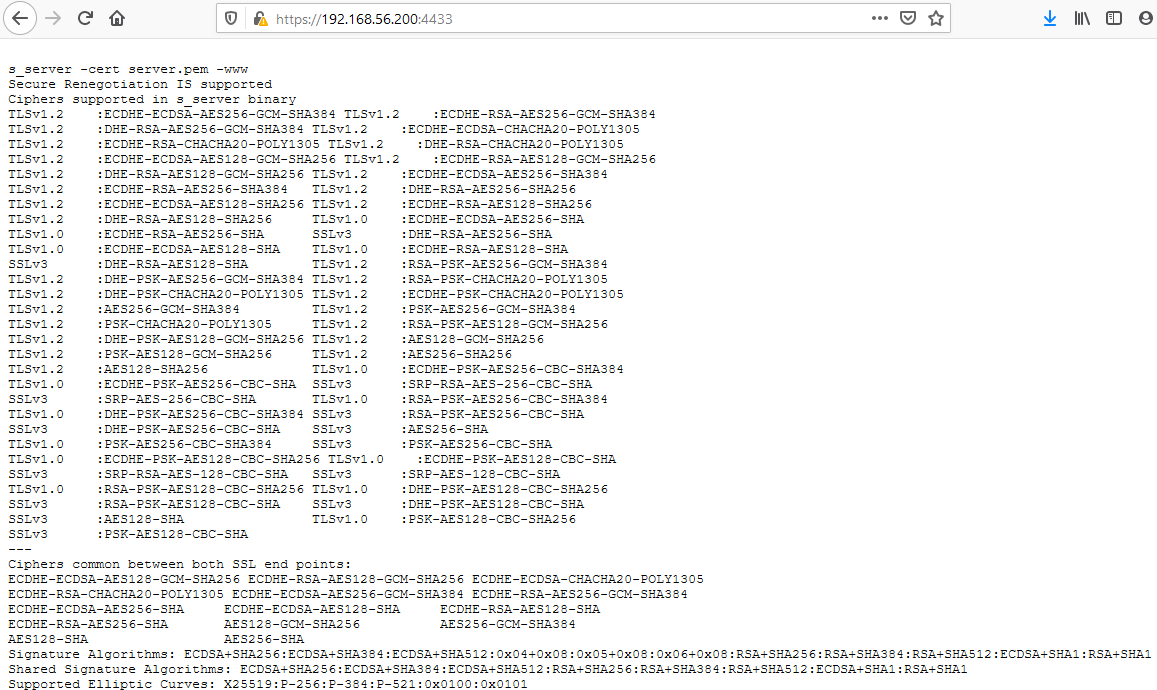
\includegraphics[scale=0.4]{images/tarea3_paso2.png}
\caption{Captura de pantalla del acceso desde el navegador web}
\label{fig:tarea3_paso2}
\end{figure}
\newpage

Si se intenta acceder utilizando \emph{curl} se obtendrá un error por conexión no segura ya que se desconoce el proveedor del certificado.\\
 
\begin{figure}[h!]
	\centering
	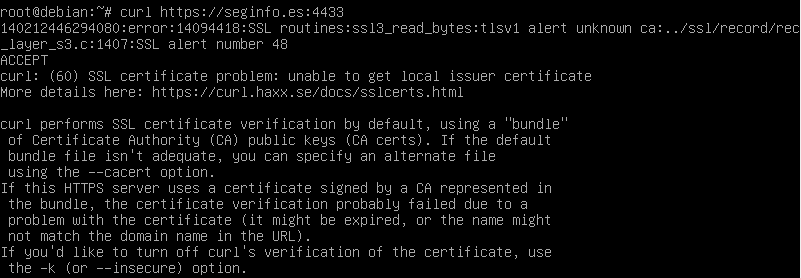
\includegraphics[scale=0.4]{images/tarea3_fallo_curl.png}
	\caption{Fallo al acceder mediante curl}
	\label{fig:tarea3_fallo_curl}
\end{figure}

Para conseguir que \emph{curl} acepte la veracidad del servidor \emph{seginfo.es} se debe añadir un argumento a la llamada:\\


\begin{lstlisting}
curl --cacert ca.crt https://seginfo.es:4433
\end{lstlisting}

Tras esto se observaría que el resultado es el mostrado en la Figura \ref{fig:tarea3_paso3}.

\begin{figure}[h!]
\centering
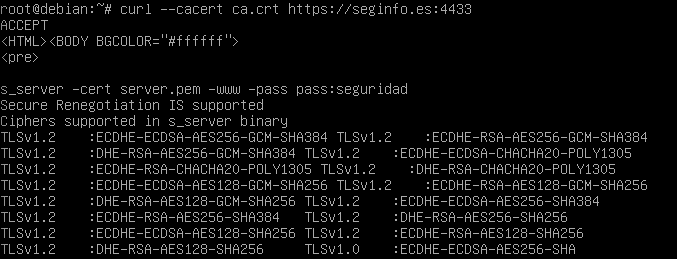
\includegraphics[scale=0.6]{images/tarea3_paso3.png}
\caption{Captura de pantalla del acceso desde curl con certificado de CA}
\label{fig:tarea3_paso3}
\end{figure}


¿Qué pasaría si modificasemos un solo byte del fichero \emph{server.pem}? Depende. Si se modifica un byte de la zona \emph{Certificate} el servidor no se inicia.\\

\begin{figure}[h!]
	\centering
	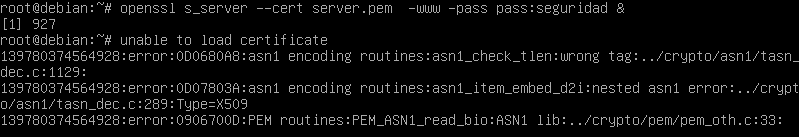
\includegraphics[scale=0.6]{images/tarea3_fallo_inicio_server.png}
	\caption{Captura de pantalla de fallo de inicio de server}
	\label{fig:tarea3_fallo_inicio_server}
\end{figure}
 Si se modifica un byte de la zona \emph{signature-algorithm} el servidor se inicia sin problemas (\textbf{No voy a meter captura, es un poco inutil no? He comprobado y si que se inicia el server}).

¿Qué ocurre si nos intentamos conectar mediante \texttt{https://localhost:4433}? Que no podremos conectar ya que el certificado ha sido emitido para \emph{seginfo.es} y no para \emph{localhost}.
\begin{figure}[h!]
	\centering
	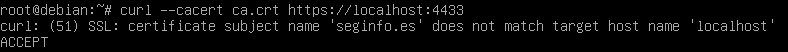
\includegraphics[scale=0.6]{images/tarea4_paso2.png}
	\caption{Captura de pantalla de fallo de inicio de server}
	\label{fig:tarea3_localhost}
\end{figure}


\section{Tarea 4: Implementación de certificados en un servidor web \emph{HTTPS} basado en \emph{Apache}}


Para configurar el servidor \textit{Apache}, se deben modificar los ficheros \textit{000-default} (para servicios \textit{Http}) y \textit{default-ssl} (servicios \textit{Https}) alojados en el directorio \texttt{/etc/apache2/sites-available}. Se debe de crear una nueva entrada que indique el nombre del servidor y la carpeta raíz donde se encuentran los archivos relacionados con el mismo. \\
\begin{figure}[h!]
	\centering
	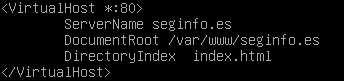
\includegraphics[scale=0.6]{images/tarea4_000default.png}
	\caption{Modificación de fichero \textit{000-default}}
	\label{fig:tarea4_000default}
\end{figure}

Para un sitio web \textit{Https}, se debe añadir un par de campos más relacionados con el certificado.\\

\begin{figure}[h!]
	\centering
	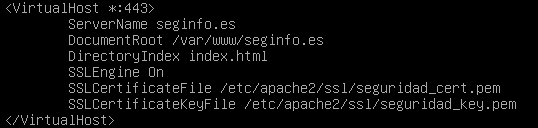
\includegraphics[scale=0.6]{images/tarea4_defaultssl.png}
	\caption{Modificación de fichero \textit{default-ssl}}
	\label{fig:tarea4_defaultssl}
\end{figure}

Posteriormente se debe crear directorio \texttt{/var/www/seginfo.es} y el fichero index.html incorporando el texto que queramos que se vea al acceder al servicio.\\
A continuación, se deben ejecutar una serie de comandos para habilitar \textit{SSL} y reiniciar el servicio Apache. Al hacerlo, se pide la introducción de la contraseña utilizada para encriptar la clave privada.\\
\begin{lstlisting}
	// Habilitar modulo SSL
	$ sudo a2enmod ssl
	// Habilitar la web anadida
	$ sudo a2ensite default-ssl
	// Comprobar si la configuracion de Apache contiene errores
	$ sudo apachectl configtest
	// Reiniciar Apache
	$ sudo systemctl restart apache2
\end{lstlisting}

Por último, se ejecuta el comando \texttt{curl --cacert ca.crt https://seginfo.es} para acceder al servicio desde la máquina y se muestra el contenido de \textit{index.html}, como se muestra en la siguiente imagen.\\
\begin{figure}[h!]
	\centering
	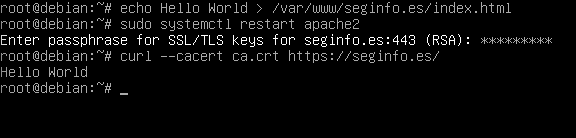
\includegraphics[scale=0.6]{images/tarea4_paso3.png}
	\caption{Modificación de fichero \textit{index.html} y acceso al servicio}
	\label{fig:tarea4_paso3}
\end{figure}


\section{Tarea 5: Lanzando un ataque \emph{MITM}}

En este apartado se va a proceder a realizar un ataque \textit{Man in The Middle (MITM)}. Para ello, se ha decidido suplantar la web \url{https://example.com}\\
Se deben seguir los pasos descritos en los puntos anteriores para poder crear el certificado del sitio a suplantar. Al finalizar se deben obtener los ficheros \texttt{example.csr, example.crt y example.key}.\\

\begin{figure}[h!]
	\centering
	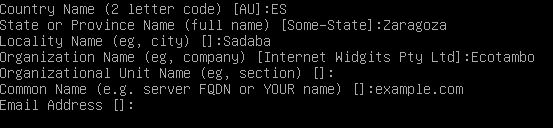
\includegraphics[scale=0.6]{images/Tarea5_paso1.png}
	\caption{Creación de certificado para example.com}
	\label{fig:tarea5_paso1}
\end{figure}
También debe modificarse las entradas \textit{VirtualHost} de \textit{Apache}, indicando como \textit{ServerName} ``example.com''. 
También se debe crear el directorio \texttt{/var/www/example.com} junto al archivo\textit{index.html}, el cual debe contener el código \textit{Html} del servicio a suplantar. En este caso se ha modificado parte del código para observar que se accede al servicio suplantado.\\
Para lanzar un MITM hay que modificar el DNS de la víctima para que en vez de acceder al servicio original, acceda a la página suplantada alojada en la máquina virutal. Para ello, se modifica el archivo \texttt{C:/Windows/System32/drivers/etc/hosts} (si la víctima es un servidor en Windows) añadiendo la siguiente entrada: ``\texttt{\_\_IP\_MV\_\_ example.com}''.\\

Si se accede a la página desde un navegador, se obtiene lo siguiente: 

\begin{figure}[h!]
	\centering
	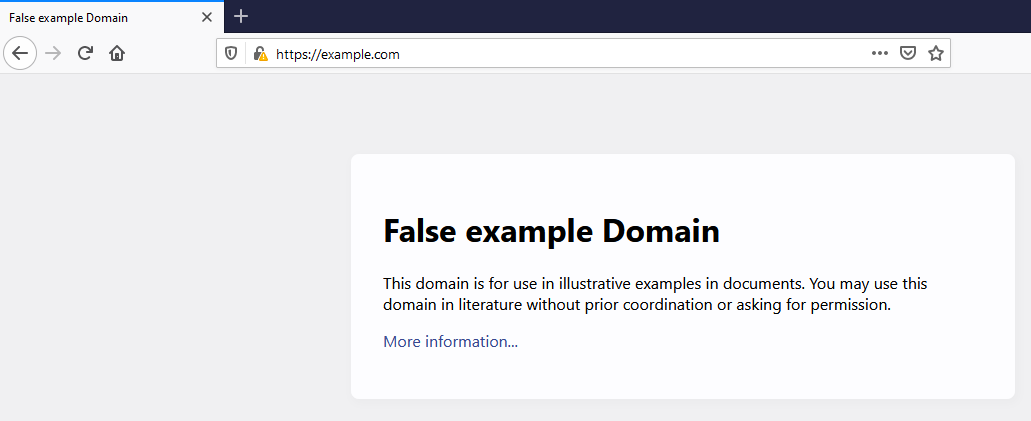
\includegraphics[scale=0.5]{images/Tarea5_paso3.png}
	\caption{Acceso a \textit{example.com } sin certificado}
	\label{fig:Tarea5_paso3}
\end{figure}

Se puede observar que el navegador indica que la conexión no es segura ya que se desconoce el certificado del emisor.\\

Para obtener una conexión segura, se debe añadir el certificado ca.crt al navegador (en este caso Firefox).\\
\begin{figure}[h!]
	\centering
	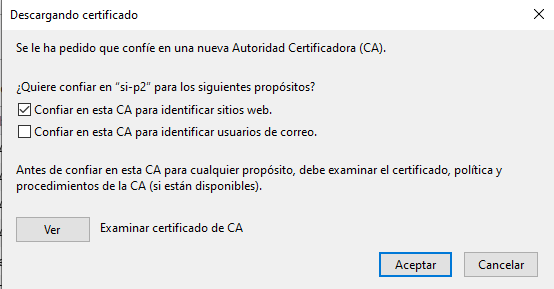
\includegraphics[scale=0.6]{images/Tarea5_paso4a.png}
	\caption{Adición de certificado a Firefox}
	\label{fig:Tarea5_paso4a}
\end{figure}

Tras añadir el certificado, se vuelve a acceder a la página y esta vez no se muestra el aviso de ``conexión no segura''\\
\begin{figure}[h!]
	\centering
	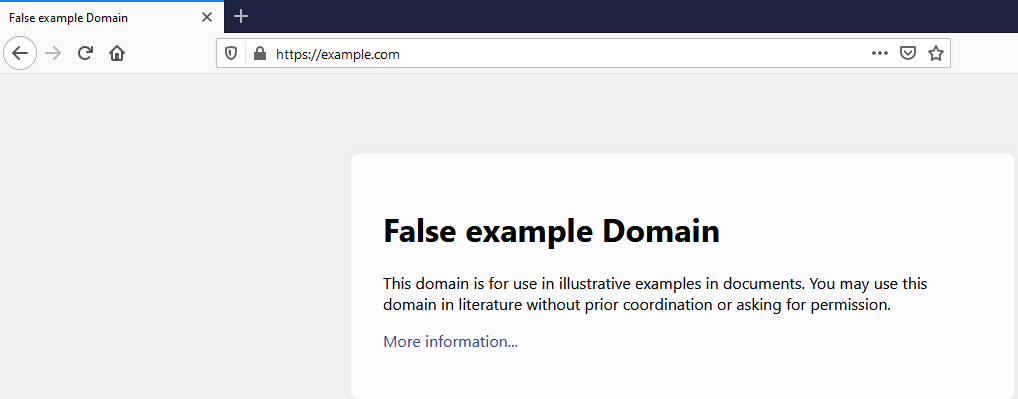
\includegraphics[scale=0.5]{images/Tarea5_paso4b.png}
	\caption{Acceso a \textit{example.com } con certificado}
	\label{fig:Tarea5_paso4b}
\end{figure}


\section{Tarea 6: Lanzando un ataque \emph{MITM} con una CA comprometida}

En este apartado, se supone un escenario en el que un atacante ha obtenido la clave privada de nuestra CA y puede crear cualquier certificado a partir de esta clave. \\
Siguiendo el escenario anterior, la víctima que había añadido el certificado a su navegador está expuesta a un ataque \textit{MITM}, ya que basta con crear un nuevo certificado para un servicio \textit{HTTPS} y realizar un ataque DNS para redirigir al servicio suplantado. De esta manera, el navegador confiaría en la página sin mostrar ninguna advertencia. \\
Se procede a realizar un nuevo ataque \textit{MITM} con una nueva página, \url{https://www.pcbox.com}. Para ello, se siguen los pasos descritos en puntos anteriores (creación de certificado, nuevo servicio en Apache y ``ataque'' DNS). \par
Si la víctima accede a esta web, se le redirigirá al servicio suplantado y el navegador no informará de ningún riesgo, tal y como se muestra en la siguiente imagen. 

\begin{figure}[h!]
	\centering
	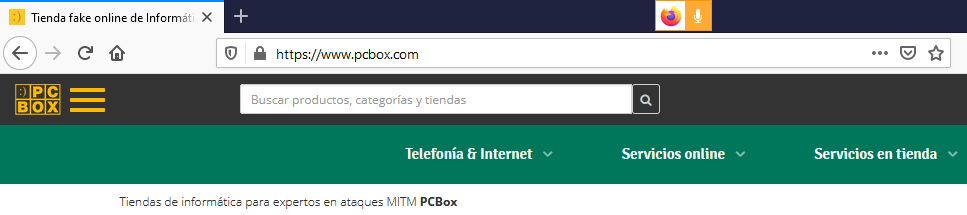
\includegraphics[scale=0.6]{images/Tarea6.png}
	\caption{Acceso a \textit{pcbox.com } falso}
	\label{fig:Tarea6}
\end{figure}


\end{document}